\documentclass[11pt]{article}

\usepackage[a4paper,margin=1in]{geometry}
\usepackage[T1]{fontenc}
\usepackage[utf8]{inputenc}
\usepackage{lmodern}
\usepackage{microtype}
\usepackage{amsmath,amssymb,amsthm,mathtools}
\usepackage{booktabs}
\usepackage{graphicx}
\usepackage{float}
\usepackage{placeins}
\usepackage{enumitem}
\usepackage[numbers,sort&compress]{natbib}
\usepackage{xcolor}
\usepackage{xurl}
\usepackage[colorlinks=true,linkcolor=blue!55!black,citecolor=blue!55!black,urlcolor=blue!55!black]{hyperref}
\usepackage[nameinlink,noabbrev]{cleveref}

\setlength{\parindent}{1.4em}
\setlength{\parskip}{0.15em}
\setlist{itemsep=0.25em,topsep=0.35em}

\newtheorem{theorem}{Theorem}[section]
\newtheorem{proposition}[theorem]{Proposition}
\newtheorem{lemma}[theorem]{Lemma}
\newtheorem{corollary}[theorem]{Corollary}
\theoremstyle{definition}
\newtheorem{definition}[theorem]{Definition}
\theoremstyle{remark}
\newtheorem{remark}[theorem]{Remark}

\newcommand{\R}{\mathbb R}
\newcommand{\C}{\mathbb C}
\newcommand{\N}{\mathbb N}
\newcommand{\uc}{u_{\mathrm c}}
\newcommand{\Id}{\mathrm I}
\newcommand{\cK}{\mathcal K}
\newcommand{\cL}{\mathcal L}
\newcommand{\cA}{\mathcal A}
\newcommand{\cR}{\mathcal R}
\newcommand{\cH}{\mathcal H}
\newcommand{\cF}{\mathcal F}
\newcommand{\spec}{\operatorname{spec}}
\newcommand{\spr}{\operatorname{spr}}
\newcommand{\cond}{\operatorname{cond}_2}

\title{\textbf{Branch-Isolated Gaussian Return Blocks}\\
\textbf{at a Quadratic Band-Merging Map:}\\[0.35em]
\large Riccati Packet Monodromy, Critical Closure, and the Bulk Spectral Edge}
\author{Liang Wang\\
\small School of Artificial Intelligence and Automation,\\[-0.2em]
\small Huazhong University of Science and Technology, Wuhan 430074, P.R. China\\
\small \texttt{wangliang.f@gmail.com}}
\date{July 2026}

\begin{document}

\maketitle

\begin{abstract}
At the first algebraic band-merging parameter of
$f_u(x)=1-u x^2$, a parity-extracted Gaussian Markov operator has a growing
small-noise resonance cloud.  A preceding deterministic construction found
the correct boundary cycle and exact roots-of-unity phases, but its raw
inverse-Jacobian basis has condition number at least of order $\lambda^k$.
Here we test the next operator-theoretic arrow: whether the actual noisy
dynamics carries an adapted cyclic return block along that cycle.

For the two-step map $S=f^2$, let $x_{k,j}$ be the ordered length-$k$
boundary cycle, $m_{k,j}=|S'(x_{k,j})|$, and
$\beta_{k,j}^2=1+f'(f(x_{k,j}))^2$.  We prove that the periodic Riccati
system
\[
 m_{k,j}^2t_{k,j}^2=t_{k,j+1}^2+\beta_{k,j}^2
\]
has a unique positive solution.  Peak-normalized Gaussian packets are then
transported exactly by every affine tangent channel with coefficient
\[
 c_{k,j}=\frac{t_{k,j+1}}
 {\sqrt{t_{k,j+1}^2+\beta_{k,j}^2}},
 \qquad
 \prod_{j=0}^{k-1}c_{k,j}=|(S^k)'(p_{2k})|^{-1}.
\]
Thus Gaussian adaptation preserves the deterministic geometric-mean radius
while removing its single exponentially large local weight.  It does not
make the problem uniformly conditioned: the canonical packet balance obeys
\[
 \liminf_{k\to\infty}
 \frac{\log\cond(D_k^{\rm G})}{k\log\lambda}\ge\frac12.
\]
At the half-logarithmic noise clock this leaves a
$\sigma^{-1/4+o(1)}$ barrier.

The final channel is genuinely non-affine.  In the critical scaling
$\delta_k/\sigma\to d$ and
$x=x_{k,k-1}+\sqrt\sigma q$, we derive the locally uniform conditioned
Gaussian--quadratic limit
\[
 \Gamma_{d,t}(q)=
 \frac{t}{\sqrt{1+t^2}}e^{-B_d(q)^2/[2(1+t^2)]}
 \frac{\Phi\!\left(\frac{\sqrt{1+t^2}}{t}
 [A_d(q)+B_d(q)/(1+t^2)]\right)}{\Phi(A_d(q))},
\]
where $A_d(q)=(\sqrt d-2\uc q)^2$ and $B_d=d-A_d$.
Its two symbolic preimages are separated, without a fitted cutoff, by the
physical partition $b=\uc^{-1/2}$.

Time-labeled restrictions of the exact nonlinear Gaussian operator form a
compact block-cyclic auxiliary operator.  We prove that every nonzero return
eigenvalue generates its complete roots-of-unity ring; positivity makes the
principal return eigenvalue simple.  Ordinary floating-point computations
at seven noise levels show that the resulting branch-isolated principal ring
locates the archived outer bulk radius to $5.64\times10^{-4}$ at
$\sigma=10^{-4}$, and its return operator is numerically close to rank one.
This is not yet a Feshbach theorem for the full Markov operator.  Controlling
excursions through the complementary space and the associated Schur
self-energy remains the decisive missing estimate.
\end{abstract}

\noindent\textbf{Keywords:} Gaussian transfer operator; Riccati equation;
block-cyclic operator; critical boundary layer; Krein--Rutman theorem;
Grushin problem; non-normal spectrum; quadratic map.

\medskip
\noindent\textbf{MSC 2020:} 37E05; 37D25; 47A10; 47B65; 47H07; 60J05;
65P30.

\section{Introduction}
\label{sec:introduction}

The small-noise spectral problem at the quadratic band-merging map has
progressed through three logically distinct constructions.  First, after
the Perron and parity modes are extracted, the deterministic bulk determinant
has a genuine local pole factor
\begin{equation}\label{eq:intro-pole}
 \widehat D_{0,\mathrm{bulk},2}(z)
 =\frac{\mathcal G(z)}{1-z^2/\lambda},
 \qquad \mathcal G(z)\ne0\quad (|z|<\lambda),
\end{equation}
so a fixed finite set of noisy resonances cannot provide a locally uniform
entire approximation through the pole
\citep{WangBoundaryLayer2026,WangBulkScattering2026}.  Second, the endpoint
Gaussian row family has intrinsic Hellinger and linear-kernel ranks
\begin{equation}\label{eq:intro-rank}
 N_\sigma=\frac{\log(1/\sigma)}{2\log\lambda}+O(1),
\end{equation}
without using a computed Markov eigenvalue
\citep{WangEndpointRank2026}.  Third, the boundary word
$CA(CB)^{k-1}$ supplies an exact time-ordered cycle.  Its deterministic
inverse-Jacobian monodromy has the edge-deflated determinant
\begin{equation}\label{eq:intro-geometric}
 \Pi_{k-1}(\rho_kz^2)
 =1+\rho_kz^2+\cdots+(\rho_kz^2)^{k-1},
 \qquad
 \rho_k=|(S^k)'(p_{2k})|^{-1/k},
\end{equation}
and hence the observed roots-of-unity phase grid
\citep{WangTimeOrdered2026}.

Those results do not yet identify a spectral block of the noisy operator.
The deterministic cycle is strongly unbalanced: one critical-return weight
is exponentially large, and the diagonal similarity to a constant cyclic
shift costs at least $c\lambda^k$.  At the rank scale
\eqref{eq:intro-rank}, this is a $\sigma^{-1/2}$ obstruction in the raw
Euclidean orbit basis.  The natural next attempt is to let Gaussian smoothing
choose the packet widths instead of imposing inverse-Jacobian amplitudes.
That is the subject of this paper.

There are two separate issues.  Along an ordinary affine noisy channel, a
Gaussian observable remains Gaussian and its width is determined by a
periodic Lyapunov--Riccati equation.  At the closing edge of the boundary
cycle, however, the source packet has physical width $O(\sqrt\sigma)$ and
straddles the quadratic critical partition.  Linearization is then invalid.
The final return must retain both the quadratic map and the normalization
caused by conditioning the state to $[-1,1]$ before folding.

\subsection*{Main results and logical status}

The paper keeps analytic statements, exact auxiliary-block algebra, and
floating-point evidence separate.

\begin{enumerate}[label=\textbf{G\arabic*.},leftmargin=3.2em]
 \item \textbf{Periodic Gaussian packet theorem.}
 For every repelling boundary cycle, the affine two-step channels admit a
 unique positive periodic width vector.  Their exact Gaussian channel
 coefficients lie in $(0,1)$ and telescope to the inverse cycle multiplier.
 Hence the adapted scalar cycle has exactly the same geometric-mean radius
 as the RH-17 deterministic monodromy.

 \item \textbf{A remaining quarter-power barrier.}
 The endpoint width converges to a positive constant, while the width at the
 critical source grows like $C_t\lambda^k$.  At the midpoint of the cycle the
 width is subexponential.  These facts imply
 $\cond(D_k^{\rm G})\ge\lambda^{k/2-o(k)}$.  Numerically the exponent tends
 to $1/2$, but only the lower bound is asserted analytically.

 \item \textbf{Conditioned critical closure.}
 The last two-step pullback has the explicit Gaussian--quadratic limit
 $\Gamma_{d,t}$.  It contains a non-removable Gaussian distribution-function
 ratio caused by state conditioning.  The profile is symmetric about the
 limiting coordinate of $b=\uc^{-1/2}$; retaining $x<b$ selects the boundary
 word's branch.

 \item \textbf{Exact root-ring algebra.}
 Time-labeled local channels
 $A_j=\chi_j\cK_\sigma^2\chi_{j+1}$ define a compact block-cyclic operator.
 Every nonzero eigenvalue $\eta$ of one full return produces all $k$ roots in
 component time and all $2k$ roots after the one-step bipartite lift.  The
 principal return is positive and simple, so its roots form the exact outer
 ring of the auxiliary block.

 \item \textbf{Seven-noise audit.}
 With $k=N_\sigma^{\rm H}+1$ selected by the independent RH-16 half-energy
 rank and with a fixed six-width window, the nonlinear local-return radius
 approaches the archived full-operator bulk edge.  The tail-three radial RMS
 error is $1.96\times10^{-3}$, compared with $1.72\times10^{-2}$ for the
 deterministic-cycle radius.  These are ordinary floating-point comparisons,
 not error-controlled spectral enclosures.

 \item \textbf{Unproved Feshbach arrow.}
 We do not prove that the branch-isolated direct-sum block is similar to, or
 is the Schur complement of, the full Gaussian Markov operator.  The sharp
 windows discard trajectories that leave and later re-enter the packet tube.
 A complement-resolvent estimate and a bound on that return self-energy are
 still required.
\end{enumerate}

The status can be summarized as
\begin{equation}\label{eq:logical-status}
 \boxed{
 \begin{gathered}
 \text{boundary cycle}
 \Longrightarrow
 \text{periodic Gaussian tube}
 \Longrightarrow
 \text{conditioned critical closure},\\
 \text{conditioned critical closure}
 \Longrightarrow
 \text{exact auxiliary root ring},\\
 \text{auxiliary root ring}
 \quad\Longrightarrow?\quad
 \text{full Markov Feshbach block}.
 \end{gathered}}
\end{equation}
The entire upper line is proved here or reduced to previously proved cycle
asymptotics.  The lower arrow is tested numerically and remains open.

\section{Boundary dynamics and the folded Gaussian operator}
\label{sec:setup}

Let $\uc$ be the root in $(1,2)$ of
\begin{equation}\label{eq:cubic}
 u^3-2u^2+2u-2=0,
\end{equation}
and set
\begin{equation}\label{eq:constants}
 f(x)=1-\uc x^2,
 \qquad r=\uc-1,
 \qquad \lambda=2\uc r.
\end{equation}
Then
\begin{equation}\label{eq:postcritical}
 0\longmapsto1\longmapsto-r\longmapsto r\longmapsto r,
\end{equation}
and
\begin{equation}\label{eq:numerical-constants}
 \uc=1.543689012692076\ldots,
 \quad r=0.543689012692076\ldots,
 \quad \lambda=1.678573510428322\ldots.
\end{equation}
Write $S=f^2$.  The component fixed point has
$S'(r)=\lambda^2$.

For $y\in[-r,1]$, define
\begin{equation}\label{eq:inverse-branches}
 g_+(y)=\sqrt{\frac{1-y}{\uc}},
 \qquad
 g_-(y)=-\sqrt{\frac{1-y}{\uc}},
\end{equation}
and
\begin{equation}\label{eq:hq}
 h=g_+\circ g_+,
 \qquad q=g_+\circ g_-.
\end{equation}
Thus $S\circ h=S\circ q=\Id$ on the corresponding branches,
$h(r)=r$, and $h'(r)=\lambda^{-2}$.

Let $p_k=p_{2k}$ be the fixed point of $q\circ h^{k-1}$ and put
\begin{equation}\label{eq:clearance}
 \delta_k=1-p_k.
\end{equation}
The boundary-cycle theorem gives
\begin{equation}\label{eq:clearance-asymptotic}
 \delta_k=C_{\rm b}\lambda^{-2k}(1+o(1)),
 \qquad
 C_{\rm b}=0.4608051492\ldots>0.
\end{equation}
Its component-time orbit is
\begin{equation}\label{eq:ordered-cycle}
 x_{k,0}=p_k,
 \qquad
 x_{k,j}=h^{k-j}(p_k)\quad(1\le j\le k-1),
\end{equation}
with
\begin{equation}\label{eq:cycle-order}
 S(x_{k,j})=x_{k,j+1\pmod k}.
\end{equation}
The multiplier satisfies
\begin{equation}\label{eq:multiplier-asymptotic}
 M_k:=(S^k)'(p_k)
 =-C_M\lambda^k(1+o(1)),
 \qquad C_M=1.9463429052\ldots>0.
\end{equation}
Equations \eqref{eq:clearance-asymptotic}--\eqref{eq:multiplier-asymptotic}
are analytic results from the preceding boundary-cycle construction; the
displayed decimals are multiprecision evaluations
\citep{WangTimeOrdered2026}.

The point
\begin{equation}\label{eq:partition-b}
 b=h(1)=\uc^{-1/2}
\end{equation}
is the source-side critical partition.  The final cycle point
$x_{k,k-1}=h(p_k)$ lies to its left and approaches it as
\begin{equation}\label{eq:last-point-scale}
 b-x_{k,k-1}
 =\frac{\sqrt{\delta_k}}{2\uc}+O(\delta_k).
\end{equation}

\subsection{The row-normalized folded kernel}

Let
\begin{equation}\label{eq:normal-density}
 \phi_\sigma(t)=\frac1{\sqrt{2\pi}\sigma}
 e^{-t^2/(2\sigma^2)},
 \qquad
 \Phi(a)=\frac1{\sqrt{2\pi}}\int_{-\infty}^a e^{-z^2/2}\,dz.
\end{equation}
For $x,y\in[0,1]$, define
\begin{align}
 Z_\sigma(x)
 &=\int_0^1\{\phi_\sigma(y-f(x))+\phi_\sigma(y+f(x))\}\,dy,
 \label{eq:normalization}\\
 P_\sigma(x,y)
 &=\frac{\phi_\sigma(y-f(x))+\phi_\sigma(y+f(x))}
 {Z_\sigma(x)}.
 \label{eq:folded-kernel}
\end{align}
The folded backward Markov operator is
\begin{equation}\label{eq:markov-operator}
 (\cK_\sigma g)(x)=\int_0^1P_\sigma(x,y)g(y)\,dy.
\end{equation}
Probabilistically, one adds $N(0,\sigma^2)$ noise to $f(x)$, conditions the
result to lie in $[-1,1]$, and then folds by absolute value.  For each fixed
$\sigma>0$, the kernel is continuous and strictly positive.  Hence
$\cK_\sigma$ and its restrictions below are compact on $L^2(0,1)$.

\section{The periodic affine Gaussian tube}
\label{sec:riccati}

Along the ordered cycle define
\begin{equation}\label{eq:m-beta}
 m_{k,j}=|S'(x_{k,j})|,
 \qquad
 \beta_{k,j}^2=1+f'(f(x_{k,j}))^2.
\end{equation}
The second formula is the variance of the two independent one-step noises
after linearizing their two-step composition.  In coordinates
$x=x_{k,j}+\sigma q$, the tangent channel has the form
\begin{equation}\label{eq:affine-channel}
 (\cL_{k,j}^{\rm aff}g)(q)
 =\int_\R g(m_{k,j}q+\beta_{k,j}z)
 \frac{e^{-z^2/2}}{\sqrt{2\pi}}\,dz.
\end{equation}
The sign of $S'$ is immaterial for centered even Gaussian observables.

\begin{theorem}[Unique periodic Riccati tube]
\label{thm:periodic-riccati}
For every $k$ for which $|M_k|>1$, there is a unique vector
$v_{k,j}=t_{k,j}^2>0$ satisfying
\begin{equation}\label{eq:riccati-recurrence}
 m_{k,j}^2v_{k,j}=v_{k,j+1}+\beta_{k,j}^2,
 \qquad j\pmod k.
\end{equation}
It is given explicitly by
\begin{equation}\label{eq:variance-explicit}
 v_{k,j}=
 \frac{1}{1-|M_k|^{-2}}
 \sum_{\ell=0}^{k-1}
 \frac{\beta_{k,j+\ell}^2}
 {\prod_{s=0}^{\ell}m_{k,j+s}^2},
\end{equation}
where all indices are cyclic.
\end{theorem}

\begin{proof}
Rewrite \eqref{eq:riccati-recurrence} as
\[
 v_{k,j}=m_{k,j}^{-2}v_{k,j+1}
 +m_{k,j}^{-2}\beta_{k,j}^2.
\]
Iterating once around the cycle gives
\[
 v_{k,j}=|M_k|^{-2}v_{k,j}
 +\sum_{\ell=0}^{k-1}
 \frac{\beta_{k,j+\ell}^2}
 {\prod_{s=0}^{\ell}m_{k,j+s}^2}.
\]
Since $|M_k|>1$, solving for $v_{k,j}$ yields
\eqref{eq:variance-explicit}, which is positive.  The difference of any two
periodic solutions would satisfy the homogeneous recurrence and therefore
would equal $|M_k|^{-2}$ times itself after one circuit; it must vanish.
\end{proof}

For this width vector, put
\begin{equation}\label{eq:gaussian-packets}
 G_{k,j}(q)=e^{-q^2/(2t_{k,j}^2)}.
\end{equation}

\begin{theorem}[Exact affine packet monodromy]
\label{thm:packet-monodromy}
The affine tangent channels transport the peak-normalized packets exactly:
\begin{equation}\label{eq:channel-identity}
 \cL_{k,j}^{\rm aff}G_{k,j+1}
 =c_{k,j}G_{k,j},
\end{equation}
where
\begin{equation}\label{eq:channel-coefficient}
 c_{k,j}
 =\frac{t_{k,j+1}}
 {\sqrt{t_{k,j+1}^2+\beta_{k,j}^2}}
 =\frac{t_{k,j+1}}{m_{k,j}t_{k,j}}
 \in(0,1).
\end{equation}
Their product is the exact inverse cycle multiplier:
\begin{equation}\label{eq:coefficient-product}
 \boxed{\prod_{j=0}^{k-1}c_{k,j}=|M_k|^{-1}.}
\end{equation}
\end{theorem}

\begin{proof}
For $m,\beta,T>0$, completing the square gives
\begin{equation}\label{eq:gaussian-integral}
 \int_\R
 e^{-(mq+\beta z)^2/(2T^2)}
 \frac{e^{-z^2/2}}{\sqrt{2\pi}}\,dz
 =\frac{T}{\sqrt{T^2+\beta^2}}
 e^{-m^2q^2/[2(T^2+\beta^2)]}.
\end{equation}
Take $T=t_{k,j+1}$ and use
\eqref{eq:riccati-recurrence}.  This proves
\eqref{eq:channel-identity}--\eqref{eq:channel-coefficient}.  Multiplication
around the cycle cancels every packet width and leaves
\[
 \prod_jc_{k,j}
 =\frac{\prod_jt_{k,j+1}}
 {\prod_jm_{k,j}t_{k,j}}
 =\frac1{|M_k|}.
\]
\end{proof}

\begin{corollary}[The radius is unchanged]
\label{cor:packet-radius}
Let $W_k^{\rm G}$ be the scalar weighted cyclic shift with local weights
$c_{k,j}$.  Its spectral radius is
\begin{equation}\label{eq:packet-radius}
 \spr(W_k^{\rm G})
 =\left(\prod_jc_{k,j}\right)^{1/k}
 =|M_k|^{-1/k}=\rho_k.
\end{equation}
Thus covariance adaptation changes the distribution of local weights but not
their geometric mean.
\end{corollary}

\subsection{Endpoint and critical-source width asymptotics}

The periodic solution is narrow at the endpoint but broad at the source of
the critical closing channel.

\begin{proposition}[Two limiting width scales]
\label{prop:width-asymptotics}
Put
\begin{align}
 v_{\rm r}&=\frac{1+\lambda^2}{\lambda^4-1}
 =\frac1{\lambda^2-1},
 \label{eq:repelling-variance}\\
 v_{\rm e}&=\frac{v_{\rm r}+1+\lambda^2}{(2\uc\lambda)^2},
 \label{eq:endpoint-variance}\\
 C_t&=\frac{\sqrt{v_{\rm e}+1}}
 {4\uc\sqrt{C_{\rm b}}}.
 \label{eq:critical-width-constant}
\end{align}
Then
\begin{equation}\label{eq:width-limits}
 t_{k,0}\longrightarrow\sqrt{v_{\rm e}}
 =0.403274090775398\ldots,
 \qquad
 \frac{t_{k,k-1}}{\lambda^k}\longrightarrow C_t
 =0.257242247329236\ldots.
\end{equation}
If $n_k=\lfloor k/2\rfloor$, then
\begin{equation}\label{eq:midpoint-width}
 \log t_{k,n_k}=o(k).
\end{equation}
In fact, the midpoint widths remain bounded above and below along each parity
subsequence.
\end{proposition}

\begin{proof}
For a fixed number of initial internal steps, the cycle points converge to
$r$.  There $m^2=\lambda^4$ and $\beta^2=1+\lambda^2$, so the attracting
backward variance recurrence has the fixed value $v_{\rm r}$ in
\eqref{eq:repelling-variance}.  Formula
\eqref{eq:variance-explicit}, together with the uniform contraction of $h$
near $r$, shows $v_{k,1}\to v_{\rm r}$: contributions from the closing edge
are divided by the squared derivative of a repelling segment whose length
tends to infinity.

At $x_{k,0}\to1$,
\[
 m_{k,0}\to|S'(1)|=2\uc\lambda,
 \qquad
 \beta_{k,0}^2\to1+\lambda^2.
\]
The $j=0$ Riccati equation therefore gives
$v_{k,0}\to v_{\rm e}$.

At the final source, the critical-return derivative theorem gives
\begin{equation}\label{eq:last-multiplier}
 m_{k,k-1}
 =4\uc\sqrt{C_{\rm b}}\,\lambda^{-k}(1+o(1)),
\end{equation}
while $f(x_{k,k-1})\to0$, and hence
$\beta_{k,k-1}^2\to1$.  The closing Riccati equation
\[
 m_{k,k-1}^2v_{k,k-1}=v_{k,0}+\beta_{k,k-1}^2
\]
proves the second limit in \eqref{eq:width-limits}.

For $n_k=\lfloor k/2\rfloor$, propagate the last variance backward using
\eqref{eq:variance-explicit}.  The Koenigs linearization of $h$ gives
\[
 \prod_{j=n_k}^{k-2}m_{k,j}
 =\lambda^{2(k-1-n_k)+O(1)}.
\]
The terminal contribution is therefore of order
$\lambda^{2k-4(k-n_k)}=e^{O(1)}$, and the accumulated noise terms form a
uniformly bounded geometric sum away from the finitely many terminal
indices.  Positivity gives the lower bound.  This proves
\eqref{eq:midpoint-width}.
\end{proof}

The last physical width has a different noise scale.  If
$k=\log(1/\sigma)/(2\log\lambda)+O(1)$, then
\begin{equation}\label{eq:physical-width-scales}
 \sigma t_{k,0}=\Theta(\sigma),
 \qquad
 \sigma t_{k,k-1}=\Theta(\sqrt\sigma).
\end{equation}
This is why the final channel sees the quadratic critical geometry.

\section{The quarter-power conditioning barrier}
\label{sec:conditioning}

Let
\begin{equation}\label{eq:packet-rho}
 \rho_k=|M_k|^{-1/k}.
\end{equation}
The canonical positive diagonal balance of the packet cycle is defined by
\begin{equation}\label{eq:packet-balance}
 d_{k,j+1}=\frac{c_{k,j}}{\rho_k}d_{k,j},
 \qquad
 D_k^{\rm G}=\operatorname{diag}(d_{k,0},\ldots,d_{k,k-1}).
\end{equation}
Equation \eqref{eq:coefficient-product} closes the recurrence, and
$(D_k^{\rm G})^{-1}W_k^{\rm G}D_k^{\rm G}$ is the constant cyclic shift of
weight $\rho_k$.

\begin{lemma}[Half-cycle product]
\label{lem:half-cycle-product}
For $n_k=\lfloor k/2\rfloor$,
\begin{align}
 \prod_{j=0}^{n_k-1}m_{k,j}
 &=\lambda^{2n_k+o(k)},
 \label{eq:partial-multiplier}\\
 \prod_{j=0}^{n_k-1}c_{k,j}
 &=\lambda^{-2n_k+o(k)}.
 \label{eq:partial-coefficients}
\end{align}
\end{lemma}

\begin{proof}
For $1\le j<n_k$, the identity $x_{k,j}=h(x_{k,j+1})$ gives
$m_{k,j}=1/h'(x_{k,j+1})$.  Applying the derivative form of the Koenigs
identity to $h^{n_k-1}$ shows
\[
 \prod_{j=1}^{n_k-1}m_{k,j}
 =\lambda^{2(n_k-1)+o(k)}.
\]
The omitted endpoint factor converges to $2\uc\lambda>0$, proving
\eqref{eq:partial-multiplier}.  Telescoping
\eqref{eq:channel-coefficient} over the same segment gives
\[
 \prod_{j=0}^{n_k-1}c_{k,j}
 =\frac{t_{k,n_k}}
 {t_{k,0}\prod_{j=0}^{n_k-1}m_{k,j}}.
\]
Use \cref{prop:width-asymptotics} to obtain
\eqref{eq:partial-coefficients}.
\end{proof}

\begin{theorem}[Packet conditioning cannot be uniform]
\label{thm:packet-conditioning}
The canonical Gaussian-packet balance satisfies
\begin{equation}\label{eq:conditioning-liminf}
 \boxed{
 \liminf_{k\to\infty}
 \frac{\log\cond(D_k^{\rm G})}{k\log\lambda}
 \ge\frac12.}
\end{equation}
Equivalently,
\begin{equation}\label{eq:conditioning-growth}
 \cond(D_k^{\rm G})\ge\lambda^{k/2-o(k)}.
\end{equation}
If
\begin{equation}\label{eq:noise-clock}
 k_\sigma=\frac{\log(1/\sigma)}{2\log\lambda}+O(1),
\end{equation}
then
\begin{equation}\label{eq:quarter-power}
 \cond(D_{k_\sigma}^{\rm G})
 \ge\sigma^{-1/4+o(1)}.
\end{equation}
\end{theorem}

\begin{proof}
Iterating \eqref{eq:packet-balance} to $n_k$ gives
\[
 \frac{d_{k,n_k}}{d_{k,0}}
 =\rho_k^{-n_k}\prod_{j=0}^{n_k-1}c_{k,j}.
\]
By \eqref{eq:multiplier-asymptotic},
$\rho_k=\lambda^{-1+o(1)}$.  Combining this with
\cref{lem:half-cycle-product} yields
\[
 \frac{d_{k,n_k}}{d_{k,0}}
 =\lambda^{-n_k+o(k)}.
\]
The ratio of the largest to the smallest diagonal entry is at least the
reciprocal of this ratio, proving
\eqref{eq:conditioning-liminf}--\eqref{eq:conditioning-growth}.  Substitution
of \eqref{eq:noise-clock} gives \eqref{eq:quarter-power}.
\end{proof}

\begin{remark}[What the adaptation achieves]
\label{rem:conditioning-interpretation}
Every local coefficient in \eqref{eq:channel-coefficient} is below one, so
the exponentially large critical-return weight of the raw inverse-Jacobian
cycle has disappeared.  The obstruction is now distributed across roughly
half of the cycle: coefficients are near $\lambda^{-2}$ during the narrow
repelling segment and near one while the broad packet contracts toward the
critical source.  The theorem proves a remaining half-exponent lower bound;
it does not prove the matching upper bound.  The numerical exponent at
$k=100$ is $0.49220$.
\end{remark}

\section{Conditioned quadratic closure of the last channel}
\label{sec:critical-closure}

The affine packet theorem is exact for the tangent model, not for the
nonlinear operator.  The distinction becomes leading order at the final
source because of \eqref{eq:physical-width-scales}.

For $d,t>0$, define
\begin{equation}\label{eq:A-B}
 A_d(q)=(\sqrt d-2\uc q)^2,
 \qquad
 B_d(q)=d-A_d(q).
\end{equation}

\begin{theorem}[Conditioned critical pullback profile]
\label{thm:critical-profile}
Let $d_\sigma\to d>0$, $t_\sigma\to t>0$, and put
\begin{equation}\label{eq:critical-scaling}
 p_\sigma=1-\sigma d_\sigma,
 \qquad
 s_\sigma=h(p_\sigma),
 \qquad
 g_\sigma(y)=
 \exp\!\left[-\frac{(y-p_\sigma)^2}{2\sigma^2t_\sigma^2}\right].
\end{equation}
Then, locally uniformly for $q\in\R$,
\begin{equation}\label{eq:profile-limit}
 (\cK_\sigma^2g_\sigma)(s_\sigma+\sqrt\sigma q)
 \longrightarrow \Gamma_{d,t}(q),
\end{equation}
where
\begin{equation}\label{eq:Gamma}
 \boxed{
 \Gamma_{d,t}(q)=
 \frac{t}{\sqrt{1+t^2}}
 \exp\!\left[-\frac{B_d(q)^2}{2(1+t^2)}\right]
 \frac{
 \Phi\!\left[
 \frac{\sqrt{1+t^2}}{t}
 \left(A_d(q)+\frac{B_d(q)}{1+t^2}\right)
 \right]}
 {\Phi(A_d(q))}.}
\end{equation}
\end{theorem}

\begin{proof}
Because $f(s_\sigma)=g_+(p_\sigma)$, Taylor expansion on compact
$q$-sets gives
\begin{equation}\label{eq:first-critical-expansion}
 f(s_\sigma+\sqrt\sigma q)
 =\frac{\sqrt\sigma}{\sqrt\uc}
 (\sqrt{d_\sigma}-2\uc q)+O(\sigma).
\end{equation}
The first noisy step is a distance of order one from the state endpoints,
so its row normalization tends to one.  Folding does not alter its square.
If $Y_1$ denotes that first folded state, then
\begin{equation}\label{eq:first-square-limit}
 \frac{\uc Y_1^2}{\sigma}
 \longrightarrow A_d(q)
\end{equation}
in probability, locally uniformly in $q$.  The first noise has size
$\sigma$, whereas the deterministic intermediate value has size
$\sqrt\sigma$; at its zero, the remaining squared noise is $O(\sigma^2)$
and still vanishes after division by $\sigma$.

Consequently the mean of the second step is
\begin{equation}\label{eq:second-mean}
 f(Y_1)=1-\sigma A_d(q)+o_{\mathbb P}(\sigma).
\end{equation}
The lower state boundary is exponentially remote.  The upper boundary
conditions the standardized second noise $Z$ to $Z\le A_d(q)+o(1)$, with
normalization $\Phi(A_d(q))$.  Since
\[
 \frac{f(Y_1)+\sigma Z-p_\sigma}{\sigma}
 =B_d(q)+Z+o_{\mathbb P}(1),
\]
dominated convergence reduces the limit to
\begin{equation}\label{eq:profile-integral}
 \Gamma_{d,t}(q)
 =\frac1{\Phi(A_d(q))}
 \int_{-\infty}^{A_d(q)}
 e^{-[B_d(q)+z]^2/(2t^2)}
 \frac{e^{-z^2/2}}{\sqrt{2\pi}}\,dz.
\end{equation}
Completing the square evaluates this integral as \eqref{eq:Gamma}.
The estimates above are uniform on compact $q$-sets, proving locally uniform
convergence.
\end{proof}

\begin{corollary}[The symbolic branch midpoint]
\label{cor:critical-midpoint}
The profile is symmetric under reflection about
\begin{equation}\label{eq:q-midpoint}
 q_{\rm b}=\frac{\sqrt d}{2\uc}:
 \qquad
 \Gamma_{d,t}(q_{\rm b}+s)
 =\Gamma_{d,t}(q_{\rm b}-s).
\end{equation}
Moreover,
\begin{equation}\label{eq:partition-coordinate}
 \frac{b-s_\sigma}{\sqrt\sigma}
 \longrightarrow q_{\rm b}.
\end{equation}
Thus the two limiting lobes are the two quadratic preimages separated by the
physical partition $b=\uc^{-1/2}$.  The boundary word selects the left branch
$x<b$.
\end{corollary}

\begin{proof}
The function $A_d(q)$ depends only on
$(q-q_{\rm b})^2$, and $B_d=d-A_d$, proving the symmetry.  Expanding
$h(1-\sigma d_\sigma)$ in \eqref{eq:last-point-scale} proves
\eqref{eq:partition-coordinate}.
\end{proof}

\begin{remark}[Why conditioning is leading order]
\label{rem:conditioning-profile}
If the upper state boundary is ignored, \eqref{eq:profile-integral} is
integrated over all $z$ and reduces to
\begin{equation}\label{eq:unconditioned-profile}
 \Gamma_{d,t}^{\rm uncond}(q)
 =\frac{t}{\sqrt{1+t^2}}
 e^{-B_d(q)^2/[2(1+t^2)]}.
\end{equation}
This drops both the numerator and denominator distribution functions.  An
affine approximation additionally replaces the quadratic $A_d$ by its
linear variation on one lobe.  Neither operation is asymptotically justified
when $d=O(1)$; the numerical audit in \cref{sec:numerics} resolves the
difference directly.
\end{remark}

\section{Branch-isolated block-cyclic return operators}
\label{sec:block-cyclic}

Fix $\sigma>0$, a component period $k$, and a window multiple $L>0$.  Let
\begin{equation}\label{eq:packet-windows}
 I_{k,j}(\sigma,L)
 =\{x\in[0,1]:|x-x_{k,j}|\le L\sigma t_{k,j}\},
\end{equation}
except that the final interval is branch isolated:
\begin{equation}\label{eq:branch-window}
 I_{k,k-1}(\sigma,L)
 =\{x:|x-x_{k,k-1}|\le L\sigma t_{k,k-1},\ x<b\}.
\end{equation}
Write $\chi_j$ for multiplication by its indicator and
$\cH_j=L^2(I_{k,j})$.  The backward local channel is
\begin{equation}\label{eq:local-channel}
 A_j=\chi_j\cK_\sigma^2\chi_{j+1}:
 \cH_{j+1}\longrightarrow\cH_j,
 \qquad j\pmod k.
\end{equation}
The time labels are part of the construction.  Even if two spatial windows
overlap, their copies in the direct sum remain distinct.

Define
\begin{equation}\label{eq:block-cyclic-operator}
 \mathfrak C_{\sigma,k}:\bigoplus_{j=0}^{k-1}\cH_j
 \longrightarrow\bigoplus_{j=0}^{k-1}\cH_j,
 \qquad
 (\mathfrak C_{\sigma,k}v)_j=A_jv_{j+1}.
\end{equation}
The return to the endpoint window is
\begin{equation}\label{eq:return-operator}
 \cR_{\sigma,k}=A_0A_1\cdots A_{k-1}:\cH_0\to\cH_0.
\end{equation}

\begin{theorem}[Exact root-ring theorem]
\label{thm:root-ring}
The operators $A_j$, $\mathfrak C_{\sigma,k}$, and
$\cR_{\sigma,k}$ are compact.  Their nonzero spectra satisfy
\begin{equation}\label{eq:root-spectrum}
 \spec(\mathfrak C_{\sigma,k})\setminus\{0\}
 =\{\zeta\in\C:\zeta^k\in
 \spec(\cR_{\sigma,k})\setminus\{0\}\}.
\end{equation}
In particular, every nonzero return eigenvalue $\eta$ generates the complete
ring
\begin{equation}\label{eq:k-root-ring}
 \zeta_\ell=\eta^{1/k}e^{2\pi i\ell/k},
 \qquad 0\le\ell<k,
\end{equation}
with the same algebraic multiplicity for each root.
\end{theorem}

\begin{proof}
Each local channel has a square-integrable continuous kernel on bounded
intervals and is therefore compact.  Direct multiplication gives
\begin{equation}\label{eq:Ck-diagonal}
 \mathfrak C_{\sigma,k}^k
 =\operatorname{diag}(\cR_0,\ldots,\cR_{k-1}),
\end{equation}
where $\cR_j=A_jA_{j+1}\cdots A_{j-1}$.  Cyclic products have the same
nonzero spectrum, including algebraic multiplicity, by repeated use of the
$AB$--$BA$ correspondence for compact operators.

If $\cR_0v_0=\eta v_0$ and $\zeta^k=\eta\ne0$, define successively
\[
 v_{k-1}=\zeta^{-1}A_{k-1}v_0,
 \quad
 v_{k-2}=\zeta^{-2}A_{k-2}A_{k-1}v_0,
 \quad\ldots.
\]
Then $v=(v_0,\ldots,v_{k-1})$ satisfies
$\mathfrak C_{\sigma,k}v=\zeta v$.  Conversely,
\eqref{eq:Ck-diagonal} sends every nonzero eigenvalue $\zeta$ to a return
eigenvalue $\zeta^k$.  The same construction for generalized eigenspaces
proves the multiplicity statement.
\end{proof}

The map $f$ exchanges two dynamical components in one step.  As in the
deterministic construction, introduce the algebraic bipartite lift
\begin{equation}\label{eq:bipartite-lift}
 \mathfrak B_{\sigma,k}
 =\begin{pmatrix}0&\Id\\ \mathfrak C_{\sigma,k}&0\end{pmatrix}.
\end{equation}
It satisfies
$\mathfrak B_{\sigma,k}^2=operatorname{diag}(\mathfrak C_{\sigma,k},
\mathfrak C_{\sigma,k})$.

\begin{corollary}[One-step ring]
\label{cor:one-step-ring}
Every nonzero return eigenvalue $\eta$ generates the $2k$ one-step values
\begin{equation}\label{eq:2k-ring}
 \mu_\ell=\eta^{1/(2k)}e^{\pi i\ell/k},
 \qquad 0\le\ell<2k.
\end{equation}
Their radius is $|\eta|^{1/(2k)}$ and their phases are exact, independent of
the rank or detailed shape of the local channels.
\end{corollary}

\begin{remark}[Normalization of the one-step lift]
\label{rem:lift-normalization}
The identity block in \eqref{eq:bipartite-lift} is an algebraic normalization,
not an identification of the separate one-step noisy channels.  More
generally, a lift with off-diagonal blocks $B$ and $C$ has determinant
controlled by $BC$ and $CB$.  The two-step return is the invariant object
used here; splitting it into physical one-step Grushin blocks is part of the
remaining global problem.
\end{remark}

\begin{theorem}[Principal return and the auxiliary outer ring]
\label{thm:principal-return}
For every fixed $\sigma,k,L$ with all windows of positive measure,
$\cR_{\sigma,k}$ has a spectral radius $\eta_0>0$ that is an algebraically
simple eigenvalue with a strictly positive eigenfunction.  Every other return
eigenvalue $\eta$ satisfies $|\eta|<\eta_0$.  Consequently the $2k$ roots of
$\eta_0$ in \eqref{eq:2k-ring} form the exact outer spectral ring of the
branch-isolated auxiliary lift.
\end{theorem}

\begin{proof}
The kernel of $\cK_\sigma^2$ is strictly positive.  Integrating products of
these kernels over the intermediate windows shows that
$\cR_{\sigma,k}$ is positivity improving on $\cH_0$.  It is compact by
\cref{thm:root-ring}.  The Jentzsch--Krein--Rutman theorem therefore gives a
positive algebraically simple spectral radius and excludes every other
eigenvalue from its peripheral circle
\citep{Schaefer1974}.  The root-ring conclusion follows from
\cref{cor:one-step-ring}.
\end{proof}

For comparison with the parity-extracted cloud, the two real roots
$\pm\eta_0^{1/(2k)}$ play the role of the distinguished edge pair and are
removed.  The remaining $2k-2$ roots have exactly the degree associated with
$k=N_\sigma+1$.

\section{Seven-noise numerical audit}
\label{sec:numerics}

The analytic results through \cref{thm:principal-return} do not depend on
the following finite computations.  The audit asks a narrower question:
does the principal eigenvalue of the branch-isolated nonlinear return have
the radial size of the already archived full-operator cloud?

\subsection{Protocol}

For each of the seven RH-15 noise levels, the folded kernel is discretized by
a row-normalized midpoint Nystr\"om matrix with
\begin{equation}\label{eq:grid-scaling}
 n\sigma=20.48.
\end{equation}
Gaussian entries beyond eight standard deviations are omitted.  The maximum
row-sum error is $5.6\times10^{-16}$.  The component period is selected before
reading a bulk radius:
\begin{equation}\label{eq:period-selection}
 k=N_\sigma^{\rm H}+1,
\end{equation}
where $N_\sigma^{\rm H}$ is the RH-16 Hellinger half-energy rank.  Every
window uses $L=6$, and only the final window receives the fixed physical cut
$x<b$.  Nine positive power iterations resolve $\eta_0$; the computed
relative residuals are at most $2.6\times10^{-9}$ and are near machine
precision except at the coarsest noise.

The comparison target is the archived \emph{bulk radius}, the largest
modulus among the automatically selected parity-extracted outer cloud.  It
is not the cloud's radial mean.  No local-return parameter is fitted to that
radius.

\subsection{The nonlinear local return reaches the edge}

\begin{table}[H]
\centering
\small
\caption{Branch-isolated principal-return radius versus the archived full
bulk edge.  The RH-17 column is the deterministic cycle radius
$|M_k|^{-1/(2k)}$.}
\label{tab:edge-audit}
\begin{tabular}{rrrrrr}
\toprule
$\sigma$ & $k$ & $\eta_0$ & local radius & RH-17 radius & bulk radius\\
\midrule
$10^{-2}$        &3&0.16523051&0.74076713&0.70350068&0.67466935\\
$4\times10^{-3}$ &4&0.09550137&0.74559194&0.71507601&0.71794136\\
$2\times10^{-3}$ &5&0.05608219&0.74969135&0.72415158&0.73627786\\
$10^{-3}$        &6&0.03022240&0.74706905&0.73108951&0.73914154\\
$5\times10^{-4}$ &6&0.03236519&0.75134577&0.73108951&0.74801500\\
$2\times10^{-4}$ &7&0.01959402&0.75510757&0.73642348&0.75474882\\
$10^{-4}$        &8&0.01149664&0.75645948&0.74059474&0.75702308\\
\bottomrule
\end{tabular}
\end{table}

At the three smallest noises, local minus full-edge errors are
\begin{equation}\label{eq:tail-errors}
 3.331\times10^{-3},
 \qquad 3.588\times10^{-4},
 \qquad -5.636\times10^{-4}.
\end{equation}
Their RMS is
\begin{equation}\label{eq:tail-rms}
 \begin{array}{c|c}
 \text{model}&\text{tail-three radial RMS}\\ \hline
 \text{nonlinear branch return}&0.0019613\\
 \text{RH-17 deterministic cycle}&0.0172451
 \end{array}
\end{equation}
The coarse-noise mismatch is substantial and is not hidden: at
$\sigma=10^{-2}$ the local block overshoots the archived edge by $0.0661$.
The evidence concerns the small-noise tail, not a uniform seven-point fit.

\begin{figure}[H]
\centering
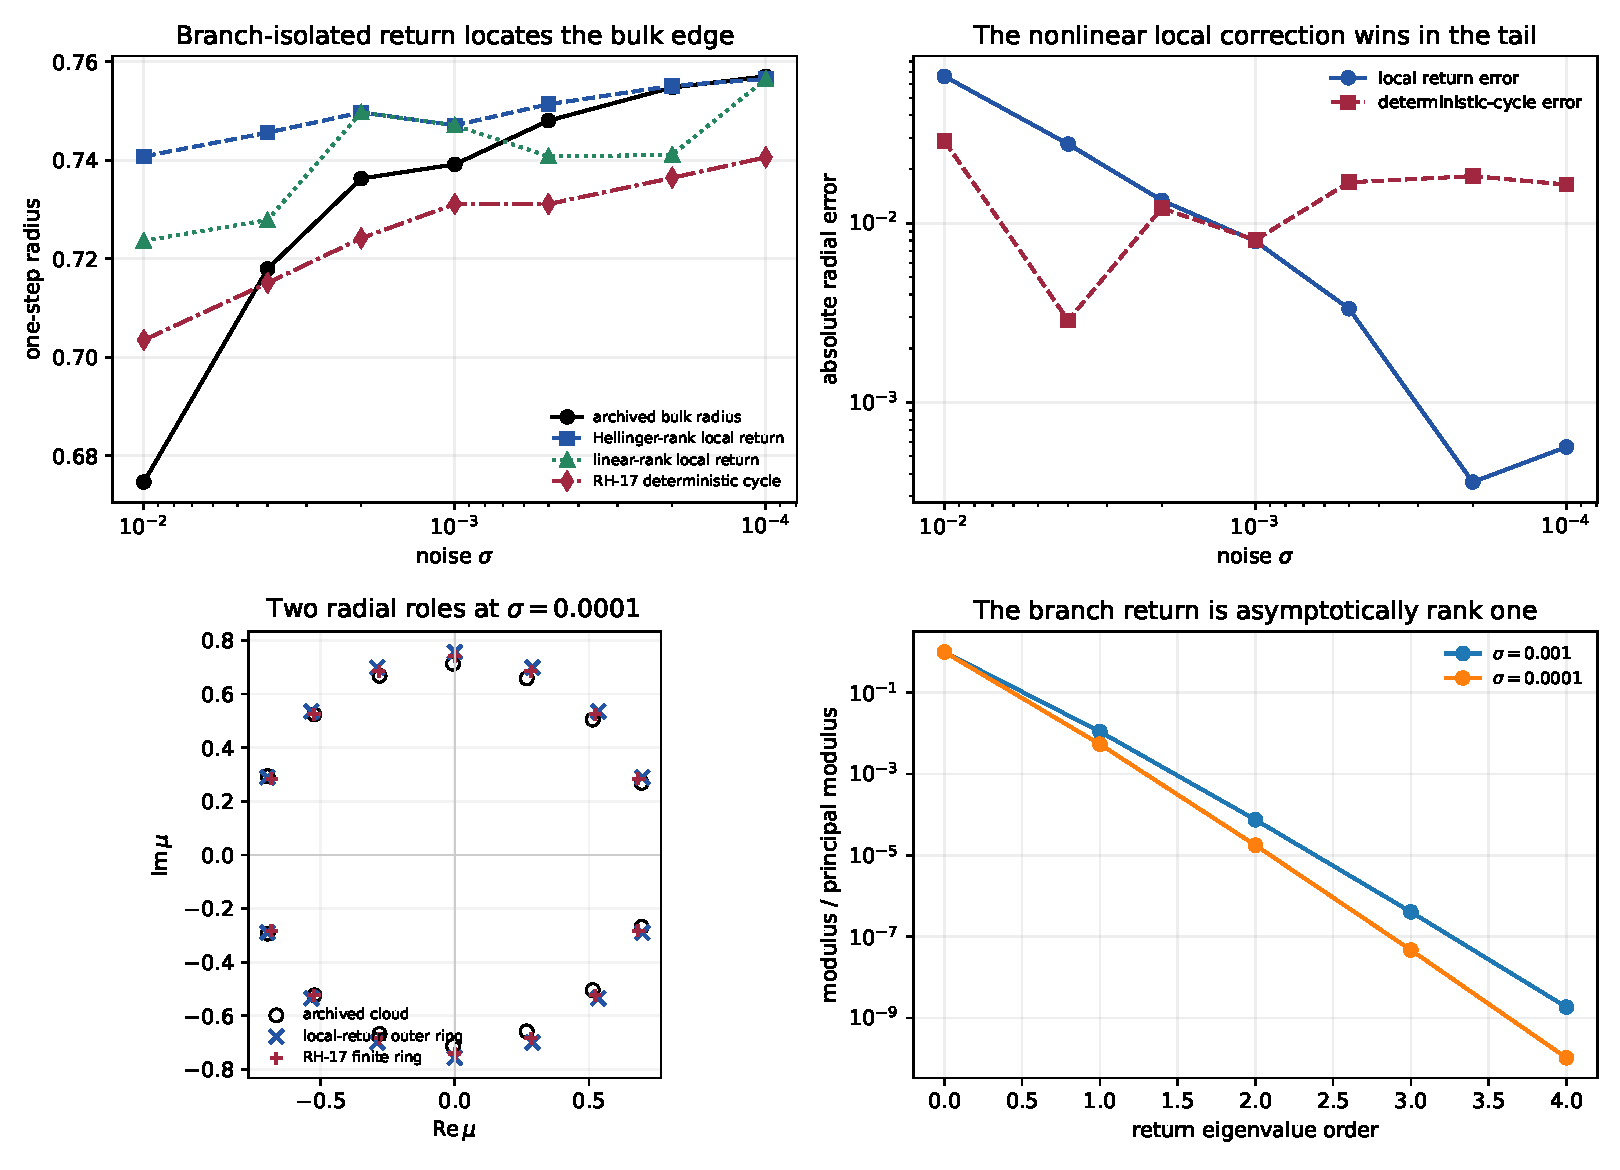
\includegraphics[width=\textwidth]{figures/branch_isolated_bulk_edge.pdf}
\caption{Branch-isolated return and full-spectrum comparison.  Top left:
the principal local-return radius selected by the Hellinger rank, the
linear-row alternative, the deterministic cycle, and the archived full
bulk edge.  Top right: absolute radial errors.  Bottom left: the smallest
noise cloud, the edge-deflated local root ring, and the RH-17 deterministic
ring.  Bottom right: moduli of the first five return eigenvalues relative to
the principal one.  All full spectra are imported unchanged from RH-15.}
\label{fig:edge-audit}
\end{figure}

The deterministic and nonlinear constructions need not have the same radial
role.  The deterministic multiplier is the first stability channel of one
orbit and previously tracked an interior finite-section radius.  The local
return includes finite-noise spreading, nonlinear closure, state
conditioning, and branch loss.  The data suggest that the latter controls
the outer edge while the former remains an interior reference.  This is an
interpretation of the audit, not an asymptotic theorem.

\subsection{The critical profile is the required local correction}

For every noise, the endpoint Gaussian is pulled back by the full sparse
$\cK_\sigma^2$ and compared on the final branch window with
\eqref{eq:Gamma}.  No amplitude is fitted for the direct error.

\begin{table}[H]
\centering
\small
\caption{Relative direct errors of the conditioned critical profile, the
unconditioned quadratic profile, and an affine Gaussian profile.}
\label{tab:critical-errors}
\begin{tabular}{rrrrr}
\toprule
$\sigma$ & $k$ & conditioned & unconditioned & affine\\
\midrule
$10^{-2}$        &3&0.050670&0.263161&0.473874\\
$4\times10^{-3}$ &4&0.025979&0.266454&0.480685\\
$2\times10^{-3}$ &5&0.013019&0.325964&0.513897\\
$10^{-3}$        &6&0.007617&0.353751&0.489578\\
$5\times10^{-4}$ &6&0.008196&0.234486&0.448693\\
$2\times10^{-4}$ &7&0.004461&0.264965&0.480745\\
$10^{-4}$        &8&0.002411&0.332190&0.511101\\
\bottomrule
\end{tabular}
\end{table}

At $\sigma=10^{-3}$, a least-squares amplitude applied only as an audit is
$1.000872$; the direct and fitted errors are $0.007617$ and $0.007567$.
Thus the agreement is not created by amplitude renormalization.  The
unconditioned and affine errors stay of order one because their omitted
terms remain leading at $\delta_k/\sigma=O(1)$.

\begin{figure}[H]
\centering
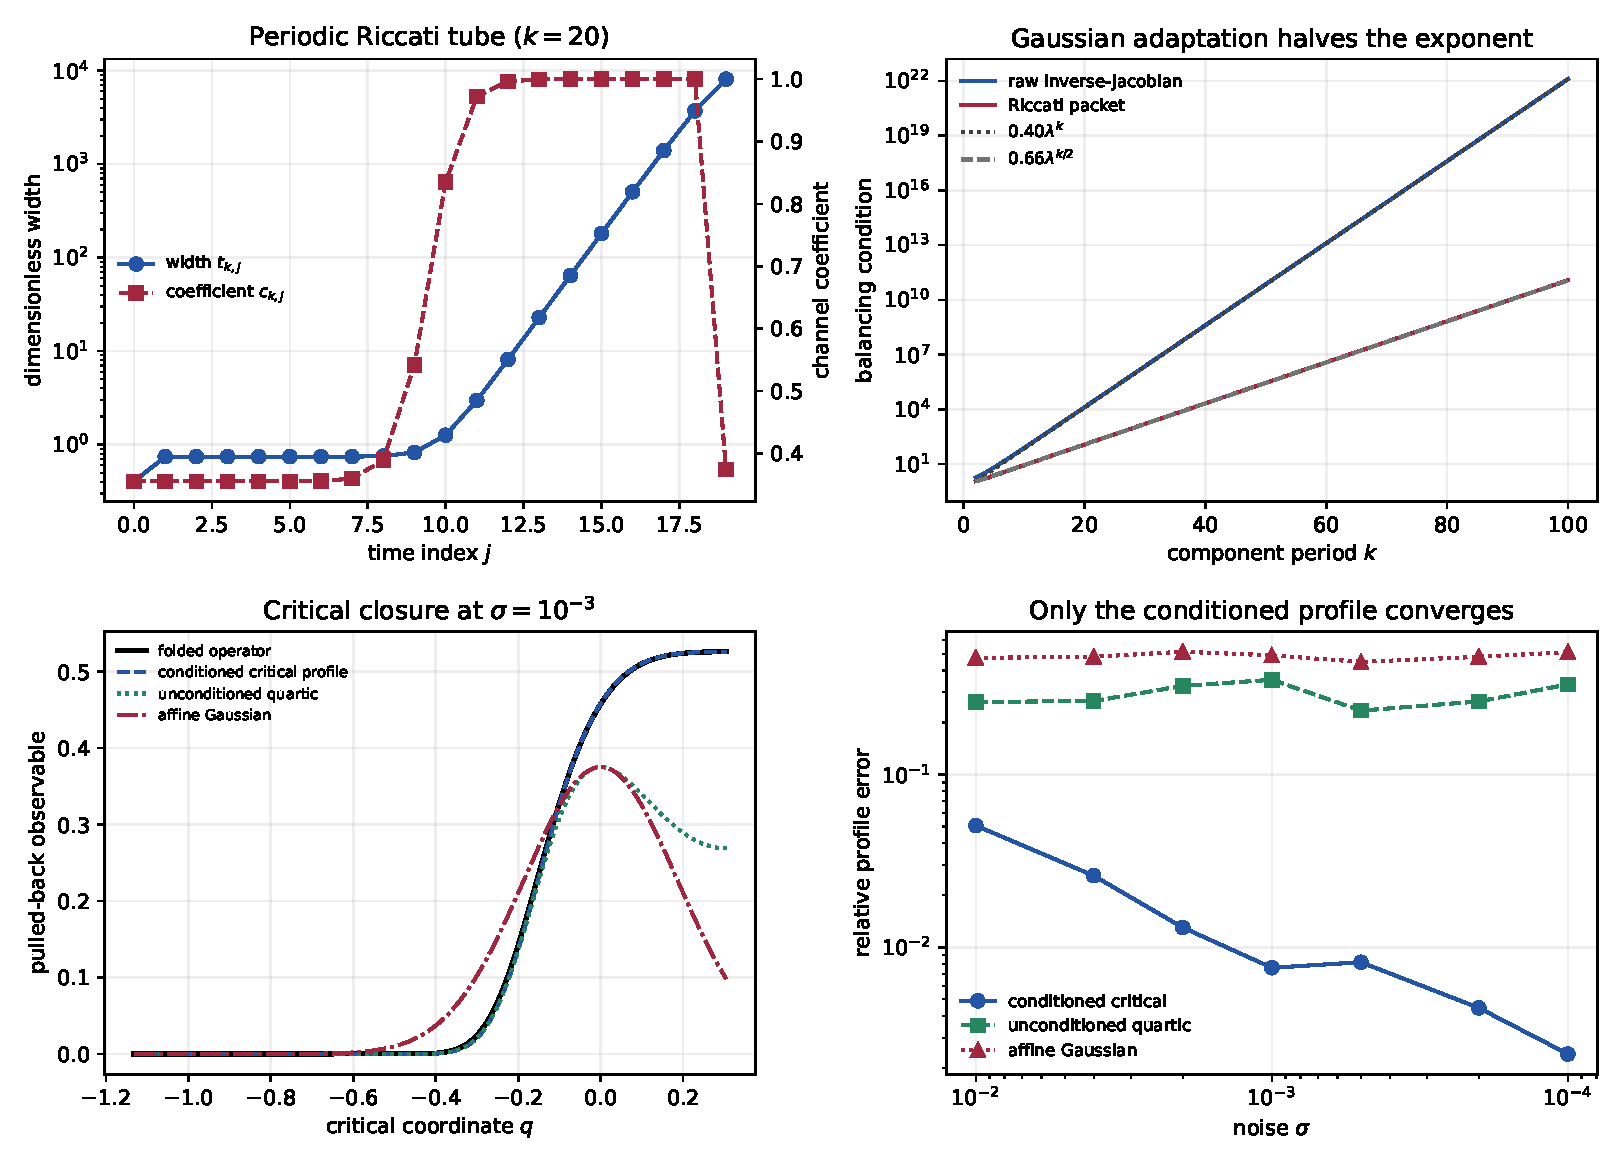
\includegraphics[width=\textwidth]{figures/riccati_packet_critical_closure.pdf}
\caption{Riccati packet and critical closure audit.  Top left: periodic
widths and affine channel coefficients at $k=20$.  Top right: raw and
Gaussian-adapted balancing conditions; the reference exponents are one and
one half.  Bottom left: the exact folded two-step pullback and three local
models at $\sigma=10^{-3}$.  Bottom right: direct profile errors at all seven
noises.}
\label{fig:riccati-critical}
\end{figure}

\subsection{Return spectral gap and discretization checks}

At $\sigma=10^{-4}$ and $k=8$, the first five computed return eigenvalue
moduli relative to $\eta_0$ are
\begin{equation}\label{eq:return-gap-data}
 1,quad
 5.398\times10^{-3},quad
 1.776\times10^{-5},quad
 4.706\times10^{-8},quad
 1.055\times10^{-10}.
\end{equation}
At $\sigma=10^{-3}$ and $k=6$, the corresponding first subleading ratio is
$1.101\times10^{-2}$.  This supports a rank-one leading return, but no
uniform small-noise singular-value theorem is inferred from two spectra.

The window audit at $\sigma=10^{-3}$ gives
\begin{equation}\label{eq:window-audit}
 \begin{array}{c|ccccc}
 L&4&5&6&8&10\\ \hline
 \eta_0^{1/(2k)}
 &0.747062438&0.747069010&0.747069051&0.747069051&0.747069051
 \end{array}
\end{equation}
so the range from four through ten widths is $6.61\times10^{-6}$.  With
$n\sigma=10.24,20.48,40.96$, the radii are respectively
\begin{equation}\label{eq:grid-audit}
 0.747075397,qquad0.747069051,qquad0.746955952.
\end{equation}
The total resolution spread is $1.19\times10^{-4}$.  This is a conventional
convergence check, not a directed-rounding bound.

\subsection{Reproducibility and numerical status}

The analytic Gaussian identities are tested against independent quadrature.
The Riccati recurrence, multiplier product, critical-profile integral,
block-cyclic spectrum, folded row normalization, branch masks, and principal
return are covered by the test suite.  NumPy, SciPy, and Matplotlib provide
the numerical implementation
\citep{HarrisEtAl2020,VirtanenEtAl2020,Hunter2007}.  The audit records
software versions, source hashes, every table row, the two return spectra,
window and grid checks, and both figures.  No interval arithmetic is used;
all decimal comparisons in this section are ordinary floating-point
evidence.

\section{What remains for a genuine Feshbach theorem}
\label{sec:feshbach}

The branch-isolated return uses the exact nonlinear Gaussian kernel, but it
is still an auxiliary operator.  At every component step it applies a sharp
window and discards the complement.  The full Markov operator allows a path
to leave the tube, travel through the bulk, and later return.  Root symmetry
inside $\mathfrak C_{\sigma,k}$ says nothing by itself about the size of
those omitted paths.

To make the distinction explicit, suppose an adapted finite-dimensional
entrance/exit construction produces a packet projection $P_\sigma$ and
$Q_\sigma=\Id-P_\sigma$.  Wherever the complement inverse exists, the
spectral Schur map contains the self-energy
\begin{equation}\label{eq:schur-self-energy}
 \Sigma_\sigma(z)
 =z^2P_\sigma\cK_\sigma Q_\sigma
 (\Id-zQ_\sigma\cK_\sigma Q_\sigma)^{-1}
 Q_\sigma\cK_\sigma P_\sigma.
\end{equation}
The branch-isolated block models the direct time-ordered return.  It does not
bound \eqref{eq:schur-self-energy}.

A global identification requires at least the following four estimates.

\begin{enumerate}[label=\textbf{F\arabic*.},leftmargin=3.1em]
 \item \textbf{Adapted packet maps.}
 Construct entrance and exit maps along all $x_{k,j}$ that include the
 non-Gaussian profile \eqref{eq:Gamma} at the closing edge.  Their Gram and
 dual-Gram bounds must be compatible with the unavoidable
 $\sigma^{-1/4+o(1)}$ balance, rather than assumed uniform in a raw Euclidean
 basis.

 \item \textbf{Complement resolvent.}
 After the Perron and parity boundary layers are removed, prove a resolvent
 bound for $Q_\sigma\cK_\sigma Q_\sigma$ on an annulus containing the bulk
 root ring.  Compactness at each fixed noise is insufficient for a uniform
 small-noise estimate.

 \item \textbf{Excursion and re-entry control.}
 Show that \eqref{eq:schur-self-energy}, including paths that cross the other
 critical branch, is small in the adapted norm on the phase-spacing scale
 $1/k$.  A Euclidean operator error alone can be amplified by the packet
 balance and does not yield eigenvalue control for this non-normal block
 \citep{Kato1995,TrefethenEmbree2005}.

 \item \textbf{Determinant comparison.}
 Prove that the residual determinant after principal-ring extraction is
 nonzero and locally normal on the target annulus.  This is needed to turn a
 collection of quasimodes into the zero count and to connect back to the
 deterministic factor \eqref{eq:intro-pole}.  A Grushin formulation is a
 natural framework for this step \citep{SjoestrandZworski2007}.
\end{enumerate}

The desired theorem would compare the full Feshbach determinant with that of
$\mathfrak B_{\sigma,k_\sigma}$ after the two real edge channels are
deflated, uniformly on contours separating consecutive roots.  Nothing in
the present numerical match proves such a contour estimate.

\section{Discussion}
\label{sec:discussion}

\subsection{What has changed since the deterministic monodromy}

The RH-17 cycle already fixed the phase mechanism: a closed time order, not a
finite unilateral shift, produces the geometric polynomial.  The present
construction inserts the actual Gaussian covariance into that time order.
The exact coefficient product shows that this insertion is compatible with
the deterministic multiplier, while the Riccati widths explain how smoothing
redistributes the extreme critical-return weight.

The redistribution is useful but incomplete.  The raw basis has a
$\lambda^k$ lower-bound barrier; the Gaussian packet basis retains at least
$\lambda^{k/2-o(k)}$.  Thus the natural normalization has moved from a
$\sigma^{-1/2}$ to a $\sigma^{-1/4+o(1)}$ obstruction at the intrinsic rank
clock.  This is a quantitative narrowing of the problem, not a proof that an
adapted Grushin reduction exists.

The critical profile is equally structural.  The width selected by the
Riccati equation reaches $O(\sqrt\sigma)$ exactly where the source approaches
$b$.  At that scale, the quadratic fold, the upper state boundary, and the
two symbolic preimages all survive in the limit.  The distribution-function
ratio in \eqref{eq:Gamma} is therefore not a finite-noise correction that can
be absorbed into a fitted amplitude.

\subsection{How far the spectral evidence reaches}

Within the auxiliary local block, the phase ring is a theorem and the
principal radius is a well-defined positive eigenvalue.  The smallest-noise
edge agreement is then a nontrivial test because the period comes from row
geometry, the branch cut comes from dynamics, and the window multiple is
held fixed.  The comparison nevertheless reuses the same Gaussian kernel
and the same state discretization as the archived full spectrum.  It should
be read as a successful localization diagnostic, not as independent
experimental confirmation.

The large return gap makes the next analysis plausible: one can try to
reduce each time-labeled channel to its principal packet plus a controlled
orthogonal remainder.  The quarter-power theorem warns that the norm in
which this is done matters.  The complement coupling in
\eqref{eq:schur-self-energy} is now the central obstruction; if it is not
small, the present direction can still fail despite the radial match.

\subsection{No arithmetic or self-adjoint spectral claim}

All operators in this paper arise from one explicit noisy quadratic map.
The roots-of-unity phases follow from finite cyclic time labels, and the
principal return is a positive compact-operator eigenvalue.  No result here
identifies these values with zeros of the Riemann zeta function, constructs a
self-adjoint Hilbert--P\'olya operator, proves a prime-power trace formula, or
implies the Riemann hypothesis.  Any arithmetic comparison would require
separate operator and trace identities not present in this work.

\section{Conclusion}

The first noisy return-block test gives a positive but deliberately limited
answer.  Along the ordered boundary cycle, affine Gaussian packets possess a
unique periodic Riccati tube and an exact monodromy whose total coefficient
is the inverse deterministic multiplier.  The adaptation removes the single
exploding local weight, but a rigorous
$\lambda^{k/2-o(k)}$ conditioning barrier remains.  The last channel cannot
be affine: its exact scaling limit is the conditioned Gaussian--quadratic
profile \eqref{eq:Gamma}, and the dynamical partition $b=\uc^{-1/2}$ selects
one of its two symbolic branches.

Restricting the full nonlinear Gaussian operator to these time-labeled branch
windows produces a compact cyclic return.  Its principal eigenvalue is simple
and generates an exact $2k$-root outer ring.  With the period selected from
the independent endpoint rank, that ring reaches the archived full bulk edge
to $5.64\times10^{-4}$ at the smallest computed noise and is numerically
separated from all subleading return rings.

What remains is also precise.  The local construction discards complement
excursions, so it is not yet the Feshbach block of the Markov operator.  The
next gate is a uniform complement-resolvent and Schur-self-energy estimate in
an adapted norm that tolerates the quarter-power balance.  Passing that gate
would convert the present exact local algebra and floating-point edge match
into a genuine noisy-cloud theorem; failing it would identify where the
boundary-cycle route ceases to control the global spectrum.

\section*{Data and code availability}

The source code, tests, CSV and JSON audits, sparse local-return spectra,
window and grid checks, figures, and manuscript are available with this
paper \citep{WangGaussianReturnCode2026}.

\bibliographystyle{plainnat}
\bibliography{references}

\end{document}
